\documentclass[twoside]{article}

%\usepackage{aistats2020}
% If your paper is accepted, change the options for the package
% aistats2020 as follows:
%
\usepackage[accepted]{aistats2020}
%
% This option will print headings for the title of your paper and
% headings for the authors names, plus a copyright note at the end of
% the first column of the first page.

% If you set papersize explicitly, activate the following three lines:
%\special{papersize = 8.5in, 11in}
%\setlength{\pdfpageheight}{11in}
%\setlength{\pdfpagewidth}{8.5in}

% If you use natbib package, activate the following three lines:
\usepackage[round]{natbib}
\renewcommand{\bibname}{References}
\renewcommand{\bibsection}{\subsubsection*{\bibname}}

% If you use BibTeX in apalike style, activate the following line:
\bibliographystyle{apalike}

% graphics
\usepackage{float}
\usepackage{graphicx}

% math and stuff
\usepackage{amssymb}
\usepackage{amsmath}
\usepackage{amsthm}
\usepackage{algorithmicx}
\usepackage{algpseudocode}
%\newcommand{\disc}{\mathrm{disc}}
%\newcommand{\cont}{\mathrm{cont}}
%\newcommand{\tr}{\mathtt{tr}}
%\newcommand{\model}{\mathcal{P}}
%\newcommand{\proposal}{\mathcal{Q}}

\begin{document}

% If your paper is accepted and the title of your paper is very long,
% the style will print as headings an error message. Use the following
% command to supply a shorter title of your paper so that it can be
% used as headings.
%
%\runningtitle{I use this title instead because the last one was very long}

% If your paper is accepted and the number of authors is large, the
% style will print as headings an error message. Use the following
% command to supply a shorter version of the authors names so that
% they can be used as headings (for example, use only the surnames)
%
%\runningauthor{Surname 1, Surname 2, Surname 3, ...., Surname n}

\twocolumn[

\aistatstitle{Automated Involutive MCMC}

\aistatsauthor{ Marco Cusumano-Towner \And Alexander K. Lew \And Vikash K. Mansinghka }

\aistatsaddress{ Massachusetts Institute of Technology } ]

\begin{abstract}
Involutive MCMC is a unifying framework for MCMC that encompasses many standard
and recent MCMC algorithms from the literature, from reversible jump MCMC to
Hamiltonian Monte Carlo to kernels based on deep neural networks. The key idea
in involutive MCMC is that a combination of (i) an auxiliary probability
distribution and (ii) an involution on the extended state space that includes
the model latent variables and the auxiliary variables results in MCMC kernels
that satisfy detailed balance with respect to the target distribution. The
involutive MCMC framework is appealing for its simplicity and generality, and
promises to be a useful conceptual and mathematical tool for exploring the
design space of MCMC kernels. However, like other Monte Carlo samplers,
implementing involutive samplers is time consuming and error prone. This paper
describes a technique for automatically generating the implementation of
involutive MCMC samplers from two probabilistic programs that define the target
distribution and the auxiliary probability distribution respectively, and a
differentiable program that defines the involution. The technique also detects
common conceptual and programming errors that arise when designing and
specifying involutive MCMC algorithms. This paper describes the support for
involutive MCMC in the Gen probabilistic system that uses this technique, and
shows involutive samplers specified using Gen's high-level probabilistic and
differentiable programming languages.
\end{abstract}

\section{INTRODUCTION}

%This is the best paper~\citep{cusumano2019gen}.

\subsection{Second Level Heading}

\subsubsection{Third Level Heading}

\paragraph{Fourth Level Heading}

\section{BACKGROUND AND RELATED WORK}

\subsection{Traces}

\begin{figure*}[ht]
    \centering
    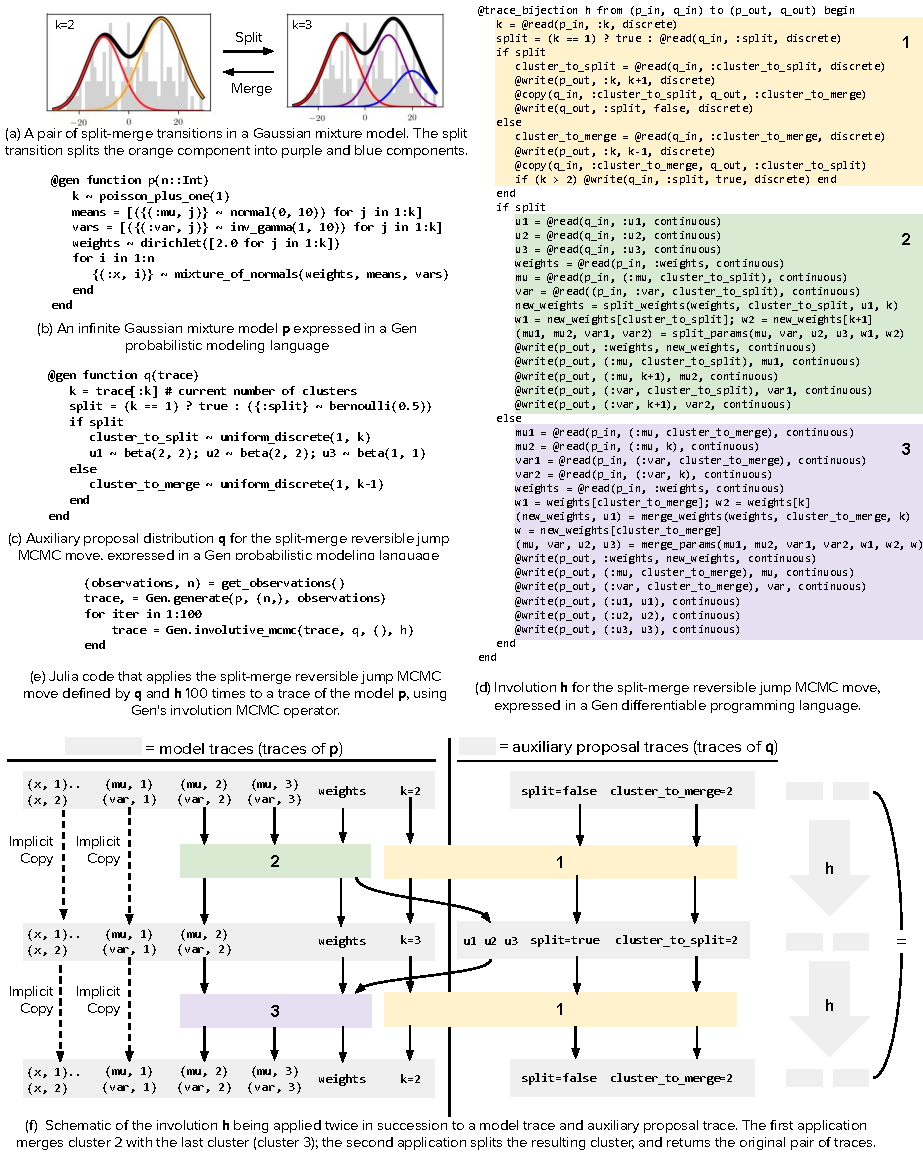
\includegraphics[width=\textwidth]{figures/mixture.pdf}
    \caption{
Example of reversible jump MCMC~\citep{green1995reversible} implemented using involutive MCMC in Gen.
The example implements a `split-merge move' in a infinite Gaussian mixture model~\citep{richardson1997bayesian} using three Gen programs:
(1) a probabilistic program $\mathtt{p}$ encoding the generative model (shown in b),
(2) a probabilistic program $\mathtt{q}$ encoding an auxiliary probability distribution (shown in c),
and (3) a differentiable program $\mathtt{h}$ that encodes an involution on the space of pairs of traces of $\mathtt{p}$ and $\mathtt{q}$ (shown in d).
Gen's involutive MCMC operator (shown in e) automatically computes the acceptance probability.
}
    \label{fig:mixture}
\end{figure*}

\begin{figure*}[ht]
    \centering
    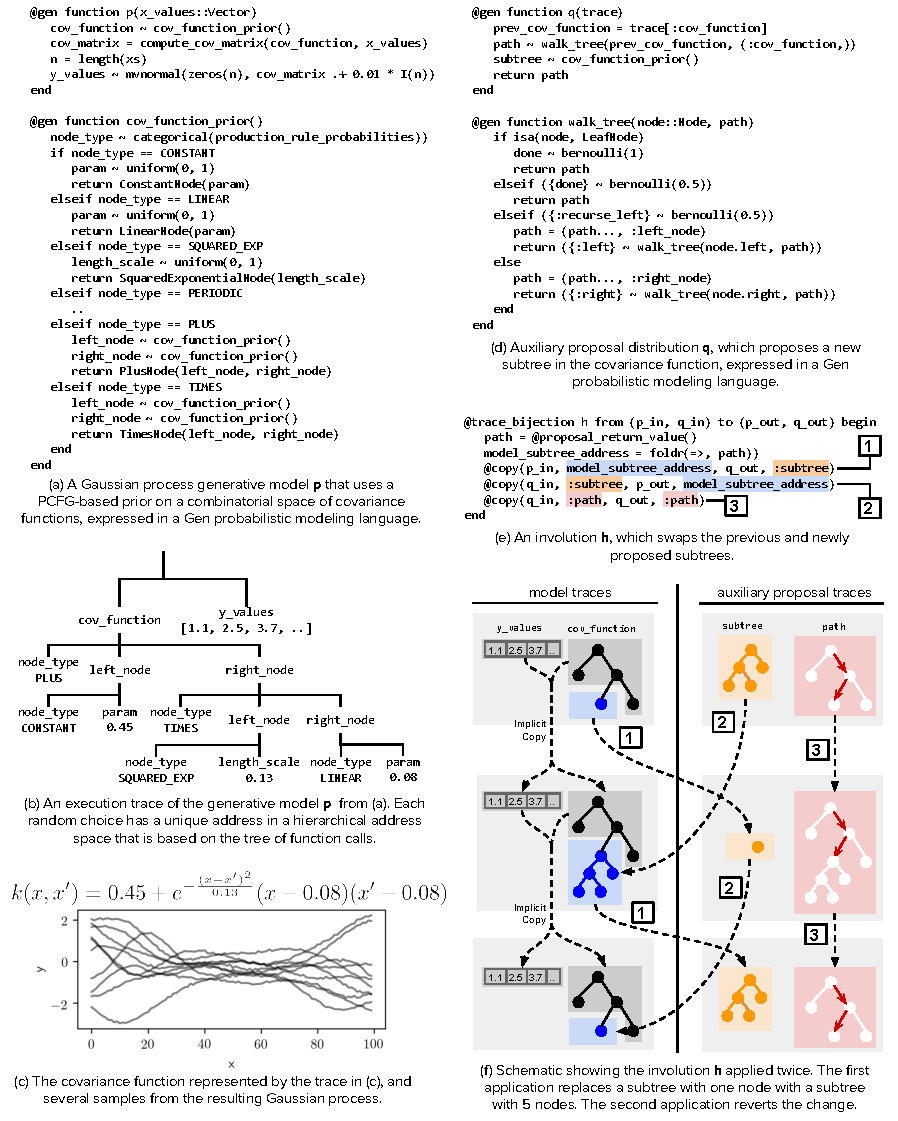
\includegraphics[width=\textwidth]{figures/structure-learning.pdf}
    \caption{
A mixture kernel implemented using involutive MCMC in Gen, applied to infer the covariance function of a Gaussian process.
The prior on covariance functions is based on a probabilistic context-free grammar.
Each component kernel in the mixture replaces a subtree of the covariance function parse tree with a new subtree.
The mixture kernel chooses a random subtree to replace via a random walk on the parse tree.
The mixture kernel is composed from three Gen programs:
(1) a probabilistic program $\mathtt{p}$ encoding the generative model (shown in a),
(2) a probabilistic program $\mathtt{q}$ encoding an auxiliary probability distribution (shown in b), and
(3) a differentiable program $\mathtt{h}$ that encodes an involution (shown in d).
}
    \label{fig:structure-learning}
\end{figure*}

\section{INVOLUTIVE MCMC WITH TRACES}

\begin{algorithmic}
\Require Target distribution $p$, proposal distribution $q$, involution $h(u, t)$, previous state $x$.
\Procedure{involutive-mcmc-move}{$p$, $q$, $f$, $x$}
    \State $u \sim q(\cdot; x)$ \Comment{Sample auxiliary variables}
    \State $(x', u') \gets f(x, u)$ \Comment{Apply involution}
    \State $\alpha \gets
        \frac{p(x') q(u'; x')}{p(x) q(u; x)} \left| \left[ \frac{\partial h(u, t)}{\partial (u, t)} \right] \right|$
    \State $r \sim \mathrm{Uniform}(0, 1)$
    \State \algorithmicif \, $r \le \alpha$ \algorithmicthen \, \Return $x'$ \algorithmicelse \, \Return $x$ 
\EndProcedure
\end{algorithmic}

% TODO PyTorch implementation??

\section{AUTOMATIC ACCEPTANCE PROBABILITY CALCULATION}

\subsection{Exploiting Jacobian Sparsity}

% TODO can only show this for a special case -- discrete involution + continuous?, or some more general case?

% TODO show an performance table of moves per second with and without the sparsity reduction (?)

\section{A DYNAMIC CHECK FOR DETECTING BUGS}

% TODO show an example of the type of bug it can detect (an edge case?)

\section{EXAMPLES}


\subsubsection*{Acknowledgements}
All acknowledgments go at the end of the paper, including thanks to reviewers who gave useful comments, to colleagues who contributed to the ideas, and to funding agencies and corporate sponsors that provided financial support.

\bibliography{references} 

\clearpage
\onecolumn
\section*{APPENDIX}

\subsection{Distributions on traces}
Define target density $\pi$ (XXX below it is called $p$, fix this) on the joint space $X \times U$, where $X$ are traces of the model and $X$ are traces of the proposal, in terms of the density $p(x)$ and the family of densities $q_x(u)$ as $\pi(x, u) := p(x) q_u(x)$.

% TODO rename the joint target density to \pi below
We want to show stationarity with respect to $\pi$, using stationarity of the involution with respect to the joint density (below).
\begin{equation}
\int_X p(x) \ell_x(A) \mu(dx) = p(A) \mbox{ for all } A \in \Sigma
\end{equation}
where $\ell_x(A)$ is the probability of transitioning into set $A$ from $x$, and is given by:
\begin{equation}
\ell_x(A) := \int_U k_{(x, u)}(A \times U) \mu(du)
\end{equation}
where $k_{(x, u)}$ is the measure on $X \times U$ that is induced by applying the involution $h$ to the state $(x, u)$.
% TODO checkme


\subsection{Stationarity of the involution with respect to joint density}
Let $(Z, \Sigma, \mu)$ be a measure space of pairs of traces of the model and proposal, where $\mu$ is $\sigma$-finite.
Consider a $\mu$-measurable function $h : Z \to Z$ that is an involution ($h(h(z)) = z$) and let $\mu \circ h^{-1}$ denote the pushforward of $\mu$ under $h$, such that $\mu \circ h^{-1}$ is $\sigma$-finite and such that $\mu \circ h^{-1}$ is absolutely continuous with respect to $\mu$.
% TODO can we simplify the conditions, using the fact that h is an involution?
Then, the Radon-Nikodym derivative exists, and is denoted $(d (\mu \circ h^{-1}) / d \mu)(z)$.

The goal is to prove stationarity with respect to the measure defined by density $p(z)$ with respect to $\mu$.
The move starts with state $z \in Z$, applies the involution $h$, and then accepts (returns $h(z)$) with probability $\alpha(z)$ and otherwise returns $z$.
Let $k_{z}$ denote the measure on new states induced by the involution $h$ and the previous state $z$:
\begin{equation}
k_{z}(A) = [h(z) \in A] \alpha(z) + [z \in A] (1 - \alpha(z))
\end{equation}
The stationarity condition is:
\begin{equation}
\int_Z p(z) k_{z}(A) \mu(dz) = p(A) = \int_Z p(z) [z \in A] \mu(dz) \mbox{ for all } A \in \Sigma
\end{equation}
Substituting in the definition of $k_z(A)$ and simplifying gives:
\begin{equation} \label{eq:stationarity-requirement}
\int_Z p(z) [h(z) \in A] \alpha(z) \mu(dz) = \int_Z p(z) [z \in A] \alpha(z) \mu(dz) \mbox{ for all } A \in \Sigma
\end{equation}
Note that for a $\mu$-measurable function $g$ such that $g \circ h$ is integrable with respect to $\mu$:
\begin{equation} \label{eq:pushforward}
\int_Z g(h(z)) \mu(dz) = \int_Z g(z) (\mu \circ h^{-1})(dz) = \int_Z g(z) \left( \frac{d (\mu \circ h^{-1})}{d \mu}(z) \right) \mu(dz)
\end{equation}
For $g(z) := p(h(z)) [z \in A] \alpha(h(z))$ we have $g(h(z)) = p(z) [h(z) \in A] \alpha(z)$, which is the integrand of the left-hand-side of Equation~(\ref{eq:stationarity-requirement}).
Applying Equation~(\ref{eq:pushforward}) to the left-hand side of Equation~(\ref{eq:stationarity-requirement}) gives:
\begin{equation}
\int_Z p(z) [h(z) \in A] \alpha(z) \mu(dz) = \int_Z g(z) \left( \frac{d (\mu \circ h^{-1})}{d \mu}(z) \right) \mu(dz) = \int_Z p(h(z)) [z \in A] \alpha(h(z)) \left( \frac{d (\mu \circ h^{-1})}{d \mu}(z) \right) \mu(dz)
\end{equation}
Equating this with the right-hand side of Equation~(\ref{eq:stationarity-requirement}) gives the following sufficient condition for stationarity:
\begin{equation}
\int_Z p(h(z)) [z \in A] \alpha(h(z)) \left( \frac{d (\mu \circ h^{-1})}{d \mu}(z) \right) \mu(dz) = \int_Z p(z) [z \in A] \mu(dz) \mbox{ for all } A \in \Sigma
\end{equation}
It therefore suffices to find $\alpha$ such that:
\begin{equation}
p(h(z)) [z \in A] \alpha(h(z)) \left( \frac{d (\mu \circ h^{-1})}{d \mu}(z) \right) = p(z) [z \in A] \alpha(z) \mbox{ for all } z \in Z
\end{equation}
The following choice of $\alpha$ suffices:
\begin{equation}
\alpha(z) = \min\left\{ 1, \frac{p(h(z))}{p(z)} \left( \frac{d (\mu \circ h^{-1})}{d \mu}(z) \right) \right\}
\end{equation}

All requirements:
\begin{enumerate}
\item $\mu$ is $\sigma$-finite
\item $h$ is $\mu$-measurable
\item $h$ is an involution
\item the pushforward $\mu \circ h^{-1}$ is $\sigma$-finite
\item the pushforward $\mu \circ h^{-1}$ is absolutely continuous with respect to $\mu$
\item the function $g(z) := p(h(z)) [z \in A] \alpha(h(z))$ is $\mu$-measurable for all $A \in \Sigma$
\item the function $(g \circ h)(z) = p(z) [h(z) \in A] \alpha(z)$ is integrable with respect to $\mu$ for all $A \in \Sigma$
\end{enumerate}

\paragraph{Characterizing the pushforward $\mu \circ h^{-1}$ for involution $h$}
Can we guarantee that it is $\sigma$-finite or absolutely continuous with respect to $\mu$?
Are there simpler sufficient conditions we can give?
$(\mu \circ h^{-1})$ is $\sigma$-finite if $Z$ is the countable union of $(mu \circ h^{-1})$-measurable sets with finite measure.

$\sigma$-finite means 


\end{document}
